\documentclass[tikz, border=1cm]{standalone}
\usepackage{pgfplots}
\pgfplotsset{compat=1.18}
\begin{document}
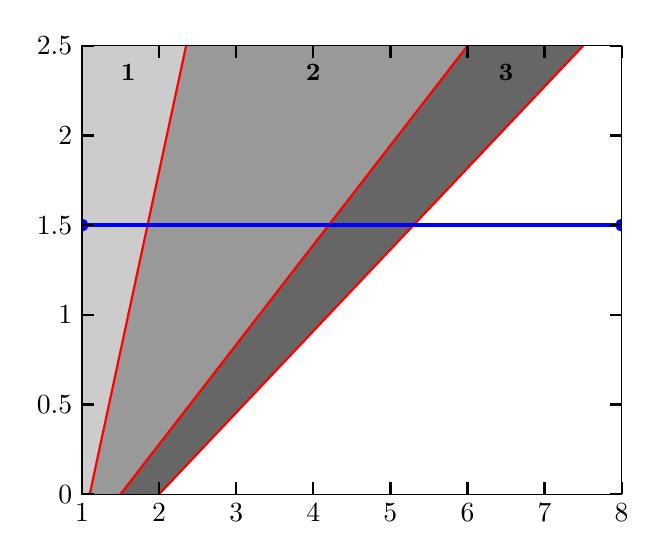
\begin{tikzpicture}[
declare function={
f1(\x)=1/0.5*(\x-1.1);
f2(\x)=1/1.8*(\x-1.5);
f3(\x)=1/2.2*(\x-2);
}]
\begin{axis}[
axis on top,
clip marker paths=true,
xmin=1, xmax=8,
ymin=0, ymax=2.5,
xtick style={black, thick},
ytick style={black, thick},
]
\fill[black!60] (1,0) -- (0,2.5) -- (8,{f3(8)}) -- (0,{f3(0)});
\fill[black!40] (1,0) -- (0,2.5) -- (8,{f2(8)}) -- (0,{f2(0)});
\fill[black!20] (1,0) -- (0,2.5) -- (8,{f1(8)}) -- (0,{f1(0)});
\addplot[red, thick, domain=1:8, samples=2] {f1(x)};
\addplot[red, thick, domain=1:8, samples=2] {f2(x)};
\addplot[red, thick, domain=1:8, samples=2] {f3(x)};
\node[font=\bf\small] at (1.6,2.350) {1};
\node[font=\bf\small] at (4.0,2.350) {2};
\node[font=\bf\small] at (6.5,2.350) {3};       
\addplot[blue, ultra thick, mark=*, mark size=1.5pt] coordinates {(1,1.5) (8,1.5)};
\end{axis}
\end{tikzpicture}
\end{document}